% Requires \usepackage{tikz}. No TikZ libraries are required.
\begin{figure}[t]
  \centering
  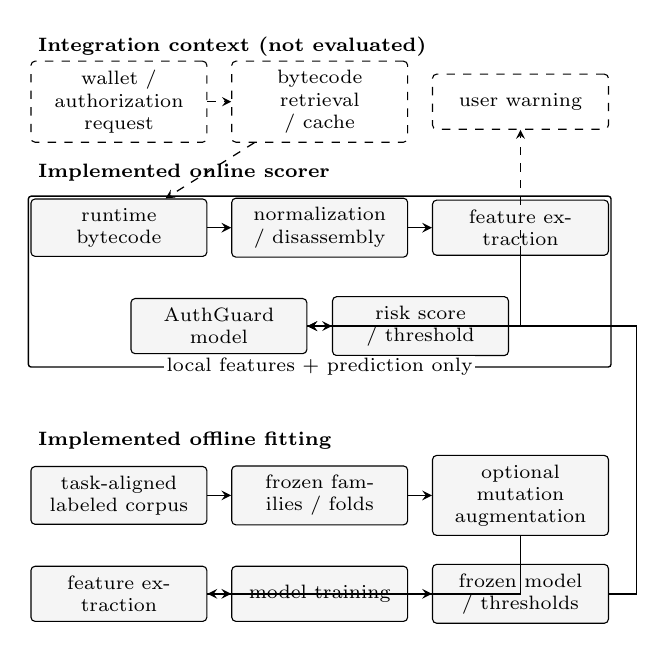
\begin{tikzpicture}[
      font=\scriptsize,
      box/.style={draw=black, rounded corners=1.5pt, minimum height=7mm,
                  text width=20mm, align=center, fill=gray!8},
      ext/.style={draw=black, dashed, rounded corners=1.5pt, minimum height=7mm,
                  text width=20mm, align=center, fill=white},
      flow/.style={draw=black, ->, >=stealth, line width=.55pt},
      context/.style={draw=black, dashed, ->, >=stealth, line width=.45pt}
    ]
    % Prospective integration context.
    \node[align=left, anchor=west] at (-3.7,8.15)
      {\textbf{Integration context (not evaluated)}};
    \node[ext] (request) at (-2.55,7.45) {wallet / authorization request};
    \node[ext] (retrieve) at (0,7.45) {bytecode retrieval / cache};
    \node[ext] (warning) at (2.55,7.45) {user warning};
    \draw[context] (request) -- (retrieve);

    % Implemented online scorer in two readable rows.
    \node[align=left, anchor=west] at (-3.7,6.55) {\textbf{Implemented online scorer}};
    \node[box] (runtime) at (-2.55,5.85) {runtime bytecode};
    \node[box] (norm) at (0,5.85) {normalization / disassembly};
    \node[box] (features) at (2.55,5.85) {feature extraction};
    \node[box] (model) at (-1.28,4.60) {AuthGuard model};
    \node[box] (decision) at (1.28,4.60) {risk score / threshold};
    \draw[context] (retrieve) -- (runtime);
    \draw[flow] (runtime) -- (norm);
    \draw[flow] (norm) -- (features);
    \draw[flow] (features.south) |- (model.east);
    \draw[flow] (model) -- (decision);
    \draw[context] (decision.east) -| (warning.south);
    \draw[line width=.5pt, rounded corners=1pt] (-3.70,4.08) rectangle (3.70,6.25);
    \node[fill=white, inner sep=1pt] at (0,4.08)
      {local features + prediction only};

    % Implemented offline fitting in two rows.
    \node[align=left, anchor=west] at (-3.7,3.15) {\textbf{Implemented offline fitting}};
    \node[box] (corpus) at (-2.55,2.45) {task-aligned labeled corpus};
    \node[box] (folds) at (0,2.45) {frozen families / folds};
    \node[box] (augment) at (2.55,2.45) {optional mutation augmentation};
    \node[box] (offfeat) at (-2.55,1.20) {feature extraction};
    \node[box] (training) at (0,1.20) {model training};
    \node[box] (frozen) at (2.55,1.20) {frozen model / thresholds};
    \draw[flow] (corpus) -- (folds);
    \draw[flow] (folds) -- (augment);
    \draw[flow] (augment.south) |- (offfeat.east);
    \draw[flow] (offfeat) -- (training);
    \draw[flow] (training) -- (frozen);
    \draw[flow] (frozen.east) -- ++(.35,0) |- (model.east);
  \end{tikzpicture}
  \caption{AuthGuard-7702 architecture. Solid nodes are implemented scorer and training paths; dashed nodes and arrows are integration context, not evaluated. The timing boundary covers only local feature construction and prediction.}
  \label{fig:system-architecture}
\end{figure}
